
\appendix
\newpage
\null\vspace{\fill} % Add vertical space before the text block

\begin{center}
	\addcontentsline{toc}{section}{APPENDIX}
	{\fontsize{14}{14}\selectfont \textbf{APPENDIX}}
\end{center}
\vspace{\fill}\null % Add vertical space after the text block

\newpage
\apendixsection{ROS2 Topics and Node Graph}
\begin{figure}[H]
    \centering
    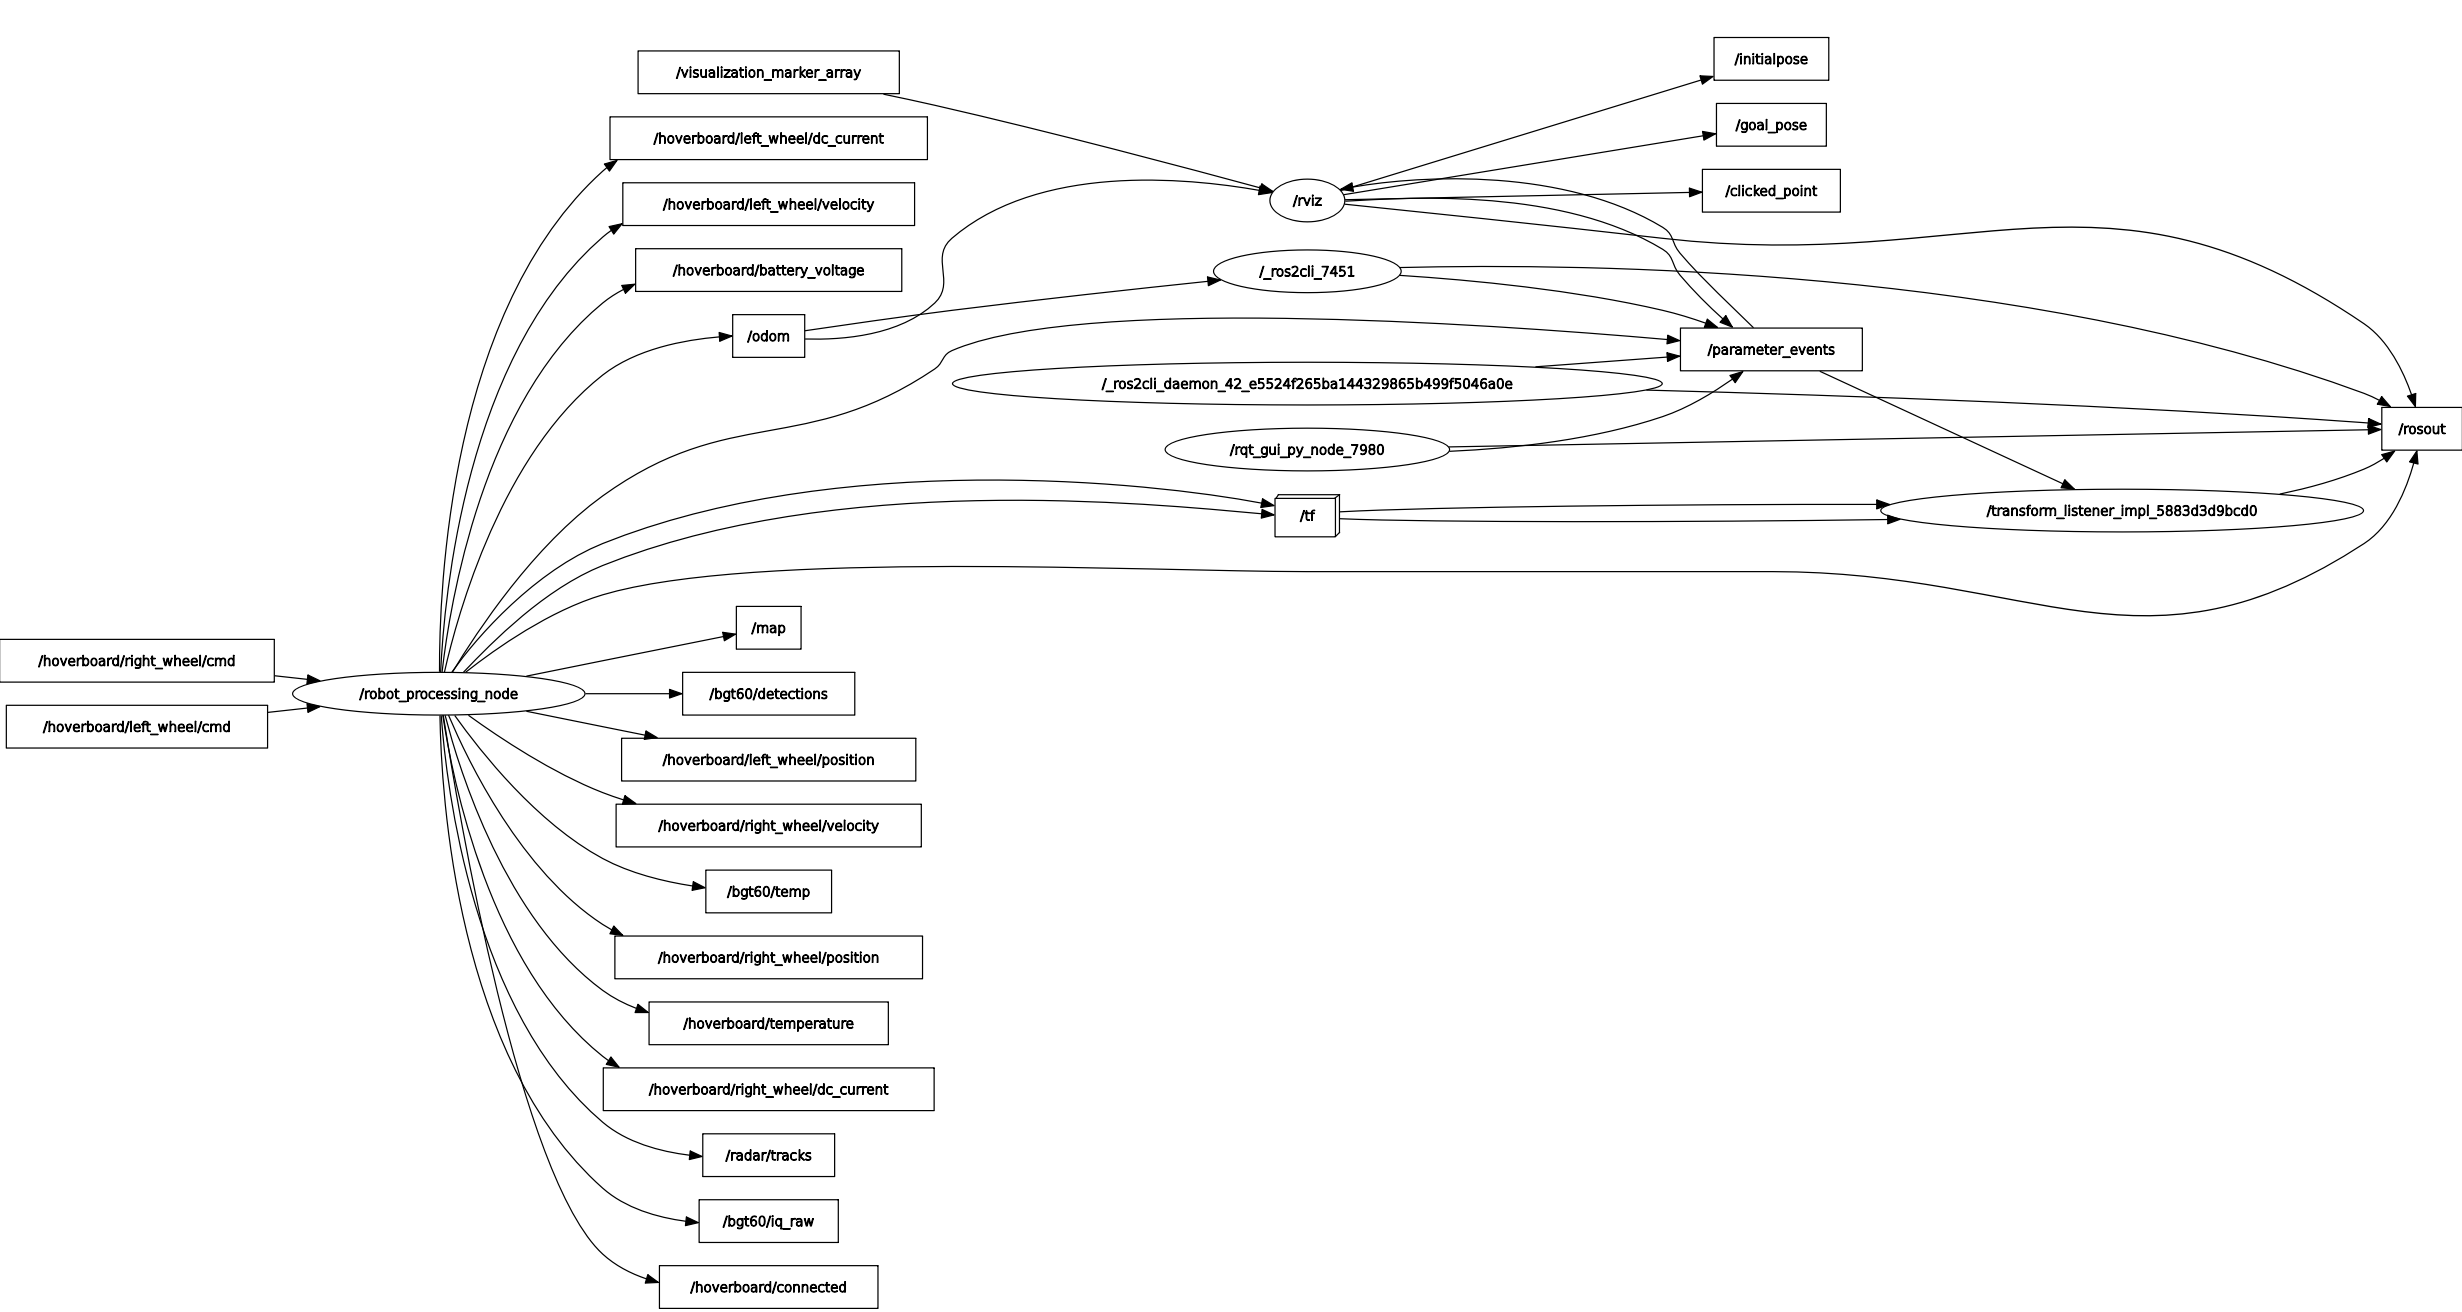
\includegraphics[angle=90, width=0.75\textwidth]{Src/images/ros2 topics.png}
    \label{fig:appendix_rotated_image}
\end{figure}




\newpage
\apendixsection{Code: Radar Initialization and Frame Acquisition}

\begin{figure}[H]
\centering
\begin{minted}[fontsize=\small,breaklines]{python}
import argparse, time, numpy as np, matplotlib.pyplot as plt
from ifxradarsdk import get_version_full
from ifxradarsdk.fmcw import DeviceFmcw
from ifxradarsdk.fmcw.types import FmcwSimpleSequenceConfig, FmcwMetrics
class BasicRadarAcquisition:
    def __init__(self):
        self.device = None
    def initialize_device(self):
        print(f"Radar SDK Version: {get_version_full()}")
        self.device = DeviceFmcw()
        print(f"Sensor: {self.device.get_sensor_type()}")
        metrics = FmcwMetrics(
            range_resolution_m=0.05, max_range_m=3.0,
            max_speed_m_s=3, speed_resolution_m_s=0.2,
            center_frequency_Hz=60_750_000_000)
        seq = self.device.create_simple_sequence(FmcwSimpleSequenceConfig())
        seq.loop.repetition_time_s = 0.2
        chirp_loop = seq.loop.sub_sequence.contents
        self.device.sequence_from_metrics(metrics, chirp_loop)
        chirp = chirp_loop.loop.sub_sequence.contents.chirp
        chirp.sample_rate_Hz = 1_000_000
        chirp.rx_mask = chirp.tx_mask = 1
        chirp.tx_power_level = 31; chirp.if_gain_dB = 33
        chirp.lp_cutoff_Hz = 500_000; chirp.hp_cutoff_Hz = 80_000
        self.device.set_acquisition_sequence(seq)
        return chirp, chirp_loop.loop.num_repetitions
    def acquire_single_frame(self):
        return self.device.get_next_frame()[0]
    def close(self):
        if self.device: self.device.close(); print("Device closed")
\end{minted}
\end{figure}

\newpage
\hfill \large Appendix 2.(continued)

\begin{figure}[H]
\centering
\begin{minted}[fontsize=\small,breaklines]{python}
    def display_frame_info(self, frame):
        print("="*60 + "\nRADAR FRAME INFORMATION\n" + "="*60)
        print(f"Shape: {frame.shape}, Dtype: {frame.dtype}")
        print(f"Antennas: {frame.shape[0]}, Chirps: {frame.shape[1]}, Samples: {frame.shape[2]}")
        print(f"Memory: {frame.nbytes} bytes")
        d = frame[0]; print(f"Min: {np.min(d)}, Max: {np.max(d)}, Mean: {np.mean(d):.2f}, Std: {np.std(d):.2f}")
    def plot_raw_data(self, frame, save_plot=False):
        fig, ax = plt.subplots(2,2,figsize=(12,8))
        d = frame[0,0,:]
        ax[0,0].plot(np.real(d), label='Real'); ax[0,0].plot(np.imag(d), label='Imag')
        ax[0,0].set_title('Single Chirp Waveform'); ax[0,0].legend(); ax[0,0].grid(True)
        ax[0,1].plot(np.abs(d)); ax[0,1].set_title('Chirp Magnitude'); ax[0,1].grid(True)
        m = np.abs(frame[0])
        im = ax[1,0].imshow(m, aspect='auto', cmap='viridis')
        ax[1,0].set_title('All Chirps Magnitude'); plt.colorbar(im, ax=ax[1,0])
        ax[1,1].plot(np.mean(m, axis=0)); ax[1,1].set_title('Avg Magnitude'); ax[1,1].grid(True)
        plt.tight_layout()
        if save_plot:
            f = f"basic_radar_data_{time.strftime('%Y%m%d_%H%M%S')}.png"
            plt.savefig(f, dpi=300, bbox_inches='tight'); print(f"Saved: {f}")
        plt.show()
\end{minted}
\end{figure}

\newpage
\hfill \large Appendix 2.(continued)

\begin{figure}[H]
\centering
\begin{minted}[fontsize=\small,breaklines]{python}
    def run_continuous_acquisition(self, num_frames=10):
        print(f"Acquiring {num_frames} frames..."); mags = []
        try:
            for i in range(num_frames):
                f = self.acquire_single_frame()
                m = np.mean(np.abs(f[0]))
                mags.append(m); print(f"Frame {i+1}: Avg = {m:.2e}")
                time.sleep(0.1)
        except KeyboardInterrupt: print("Interrupted")
        return mags
def parse_arguments():
    p = argparse.ArgumentParser(description='Basic Radar Tutorial')
    p.add_argument('--frames', '-f', type=int, default=5)
    p.add_argument('--save-plot', '-s', action='store_true')
    return p.parse_args()
def main():
    args = parse_arguments()
    radar = BasicRadarAcquisition()
    try:
        chirp_cfg, chirps = radar.initialize_device()
        print(f"Chirps/frame: {chirps}, Samples: {chirp_cfg.num_samples}")
        f = radar.acquire_single_frame(); radar.display_frame_info(f)
        radar.plot_raw_data(f, save_plot=args.save_plot)
        mags = radar.run_continuous_acquisition(args.frames)
        print(f"Avg: {np.mean(mags):.2e}, Std: {np.std(mags):.2e}, Min: {np.min(mags):.2e}, Max: {np.max(mags):.2e}")
    except Exception as e: print(f"Error: {e}")
    finally: radar.close()
if __name__ == '__main__': main()
\end{minted}
\end{figure}



\newpage
\apendixsection{Code: Range FFT Initialization and Processor Setup}

\begin{figure}[H]
\centering
\begin{minted}[fontsize=\small,breaklines]{python}
import numpy as np, matplotlib.pyplot as plt, time
from scipy import signal
from scipy.constants import c
from helpers.fft_spectrum import fft_spectrum
class RangeFFTProcessor:
    def __init__(self, chirp_cfg, num_chirps, max_r=3.0):
        self.cfg = chirp_cfg; self.n = num_chirps; self.max_r = max_r
        self.bw = abs(chirp_cfg.end_frequency_Hz - chirp_cfg.start_frequency_Hz)
        N = chirp_cfg.num_samples * 2
        self.res = c / (2 * self.bw)
        self.bin_len = c / (2 * self.bw * N / chirp_cfg.num_samples)
        self.axis = np.linspace(0, max_r, chirp_cfg.num_samples)
        try:
            self.win = signal.blackmanharris(chirp_cfg.num_samples).reshape(1, -1)
        except:
            self.win = signal.windows.blackmanharris(chirp_cfg.num_samples).reshape(1, -1) 
    def detect_peaks(self, profile, min_d=0.2, thresh_k=3.0):
        min_bin = int(min_d / self.bin_len)
        r = profile[min_bin:]; x = self.axis[min_bin:]
        if not len(r): return [], []
        t = np.mean(r) * thresh_k
        peaks, _ = signal.find_peaks(r, height=t, distance=10, prominence=t/2)
        d = x[peaks]; a = r[peaks]; s = np.argsort(a)[::-1]
        return d[s], a[s]

\end{minted}
\end{figure}

\newpage
\hfill \large Appendix 3.(continued)

\begin{figure}[H]
\centering
\begin{minted}[fontsize=\small,breaklines]{python}
    def compute_fft(self, chirps):
        rfft = fft_spectrum(chirps, self.win)
        abs_fft = np.abs(rfft)
        return np.mean(abs_fft, axis=0), abs_fft
    def calc_targets(self, d, a):
        return [{
            'target_id': i+1, 'distance_m': x, 'amplitude': y,
            'range_bin': int(x / self.bin_len),
            'signal_strength_db': 20*np.log10(y) if y > 0 else -np.inf
        } for i, (x, y) in enumerate(zip(d, a))]
    def plot(self, profile, d, a, save=False, show=True):
        fig, (ax1, ax2) = plt.subplots(2, 1, figsize=(12,8))
        ax1.plot(self.axis, profile, 'b-', label='Profile'); ax1.axvline(x=0.2, color='r', ls='--')
        if len(d):
            ax1.plot(d, a, 'ro')
            [ax1.annotate(f'T{i+1}\\n{x:.2f}m', xy=(x, y), xytext=(10, 10),
            textcoords='offset points', fontsize=10,
            bbox=dict(boxstyle='round', facecolor='yellow', alpha=0.7))
            for i, (x, y) in enumerate(zip(d, a))]
        ax1.set_xlim(0, self.max_r); ax1.grid(True); ax1.legend(); ax1.set_title('Linear')
        db = 20*np.log10(profile + 1e-10)
        ax2.plot(self.axis, db, 'g-'); ax2.axvline(x=0.2, color='r', ls='--')
        if len(d): ax2.plot(d, 20*np.log10(a), 'ro')
        ax2.set_xlim(0, self.max_r); ax2.grid(True); ax2.legend(); ax2.set_title('Log Scale')
        plt.tight_layout()
        if save:
            fn = f"range_profile_{time.strftime('%Y%m%d_%H%M%S')}.png"
            plt.savefig(fn, dpi=300); print(f"Saved: {fn}")
        if show: plt.show(); else: plt.close()
\end{minted}
\end{figure}

\newpage
\hfill \large Appendix 3.(continued)

\begin{figure}[H]
\centering
\begin{minted}[fontsize=\small,breaklines]{python}

    def analyze(self, frame, i=0, verbose=True):
        d, a = self.compute_fft(frame[i])
        p, q = self.detect_peaks(d)
        info = self.calc_targets(p, q)
        if verbose:
            print(f"\\nAnalysis (Antenna {i})\\nDetected: {len(info)}")
            for t in info:
                print(f"T{t['target_id']}: {t['distance_m']:.3f} m, "
                      f"Amp: {t['amplitude']:.2e}, SNR: {t['signal_strength_db']:.1f} dB")
        return {'range_profile': d, 'range_fft_abs': a,
                'peak_distances': p, 'peak_amplitudes': q, 'target_info': info}
\end{minted}
\end{figure}


\newpage
\apendixsection{Code: SNR Calculator Initialization}

\begin{figure}[H]
\centering
\begin{minted}[fontsize=\small,breaklines]{python}
import numpy as np, matplotlib.pyplot as plt, time
from scipy import signal
from scipy.constants import c, k, pi
from helpers.fft_spectrum import fft_spectrum
def db2lin(db): return 10**(db/10)
def lin2db(lin): return 10*np.log10(lin)
class SNRCalculator:
    def __init__(self, cfg, N, params=None):
        self.cfg, self.num_chirps = cfg, N
        p = params or {}
        self.P_t = p.get('tx_power_w', 1.4e6)
        self.G_tx_db = p.get('tx_gain_db', 33)
        self.G_rx_db = p.get('rx_gain_db', 33)
        self.G_tx, self.G_rx = db2lin(self.G_tx_db), db2lin(self.G_rx_db)
        self.f_center = (cfg.start_frequency_Hz + cfg.end_frequency_Hz) / 2
        self.wavelength = c / self.f_center
        self.bandwidth = abs(cfg.end_frequency_Hz - cfg.start_frequency_Hz)
        self.T_sys = p.get('system_temp_k', 950)
        self.L_sys_db = p.get('system_loss_db', 8)
 
\end{minted}
\end{figure}
\newpage
\hfill \large Appendix 4.(continued)

\begin{figure}[H]
\centering
\begin{minted}[fontsize=\small,breaklines]{python}
        self.L_sys = db2lin(self.L_sys_db)
        self.noise_figure_db = p.get('noise_figure_db', 10)
        self.noise_figure = db2lin(self.noise_figure_db)
        self.default_rcs = p.get('default_rcs_m2', 1.0)
        fft_size = cfg.num_samples * 2
        self.range_bin_length = c / (2 * self.bandwidth * fft_size / cfg.num_samples)
        self.max_range_m = p.get('max_range_m', 3.0)
        self.range_axis = np.linspace(0, self.max_range_m, cfg.num_samples)
        self.range_window = signal.windows.blackmanharris(cfg.num_samples).reshape(1, cfg.num_samples)
    def calculate_theoretical_snr(self, R, rcs=None):
        rcs = rcs or self.default_rcs
        num = self.P_t * self.G_tx * self.G_rx * (self.wavelength**2) * rcs
        den = ((4*pi)**3) * (R**4) * k * self.T_sys * self.bandwidth * self.L_sys * self.noise_figure
        snr_lin = num / den
        snr_db = lin2db(snr_lin)
        gain_db = lin2db(self.num_chirps)
        return snr_db, snr_db + gain_db, gain_db

    
\end{minted}
\end{figure}
\newpage
\hfill \large Appendix 4.(continued)

\begin{figure}[H]
\centering
\begin{minted}[fontsize=\small,breaklines]{python}
    def estimate_noise_floor(self, profile, start_m=2.5, end_m=3.0):
        s_bin = int(start_m / self.range_bin_length)
        e_bin = int(end_m / self.range_bin_length)
        if s_bin >= len(profile) or e_bin >= len(profile):
            s_bin = int(0.8 * len(profile))
            e_bin = len(profile)
        noise = profile[s_bin:e_bin]
        return {
            'mean': np.mean(noise), 'median': np.median(noise),
            'std': np.std(noise), 'min': np.min(noise),
            'samples': noise,
            'region_start_m': s_bin * self.range_bin_length,
            'region_end_m': e_bin * self.range_bin_length
        }
    def calculate_practical_snr(self, profile, targets, noise):
        results = []
        for d in targets:
            b = int(d / self.range_bin_length)
            if 0 <= b < len(profile):
                sig = profile[b]; noise_p = noise['mean']
                snr = sig / noise_p
                results.append({
                    'distance_m': d, 'signal_power': sig,
                    'noise_power': noise_p,
                    'snr_linear': snr, 'snr_db': lin2db(snr)
                })
        return results


        }
\end{minted}
\end{figure}


\newpage
\hfill \large Appendix 4.(continued)

\begin{figure}[H]
\centering
\begin{minted}[fontsize=\small,breaklines]{python}
    def analyze_snr_vs_distance(self, rng=(0.2, 3.0), pts=50, rcs=None):
        d = np.linspace(rng[0], rng[1], pts)
        s1, s2, g = [], [], []
        for x in d:
            a, b, g0 = self.calculate_theoretical_snr(x, rcs)
            s1.append(a); s2.append(b); g.append(g0)
        return {
            'distances': d,
            'snr_single_chirp_db': np.array(s1),
            'snr_integrated_db': np.array(s2),
            'coherent_gain_db': g[0]
    def print_snr_summary(self, res):
        print("\\nSNR Summary\\n" + "="*50)
        n, p = res['noise_info'], res['practical_snr']
        print(f"TX Power: {self.P_t/1e6:.1f} MW, Freq: {self.f_center/1e9:.2f} GHz")
        print(f"BW: {self.bandwidth/1e9:.2f} GHz, Gains: TX={self.G_tx_db} RX={self.G_rx_db} dBi")
        print(f"Temp: {self.T_sys} K, Integration: {self.num_chirps} chirps ({lin2db(self.num_chirps):.1f} dB)")
        print(f"Noise region: {n['region_start_m']:.2f}-{n['region_end_m']:.2f} m, Mean noise: {lin2db(n['mean']):.1f} dB")
        if p:
            print("\\nTarget SNR:")
            for i, r in enumerate(p):
                th = self.calculate_theoretical_snr(r['distance_m'])[1]
                print(f"Target {i+1}: {r['distance_m']:.2f} m, Signal: {lin2db(r['signal_power']):.1f} dB, "
                      f"SNR: {r['snr_db']:.1f} dB vs Theory: {th:.1f} dB → Δ = {r['snr_db'] - th:.1f} dB")
\end{minted}
\end{figure}
